\subsection{Overview}

\begin{frame}{Sequential Containers}
    The standard library provides the following sequential containers:
    \begin{center}
        \begin{tabular}{|ll|}
            \hline
            \ttt{vector} & Flexible-size array.\\
            \ttt{deque} & Double-ended queue.\\
            \ttt{list} & Doubly-linked list.\\
            \ttt{forward\_list} & Singly-linked list.\\
            \ttt{array} & Encapsulation of built-in array.\\
            \ttt{string} & A specialized container containing characters.\\
            \hline
        \end{tabular}
    \end{center}
\end{frame}

\begin{frame}{Consistent Interfaces}
    \begin{figure}[h]
        \centering
        \begin{minipage}{0.48\textwidth}
            \centering
            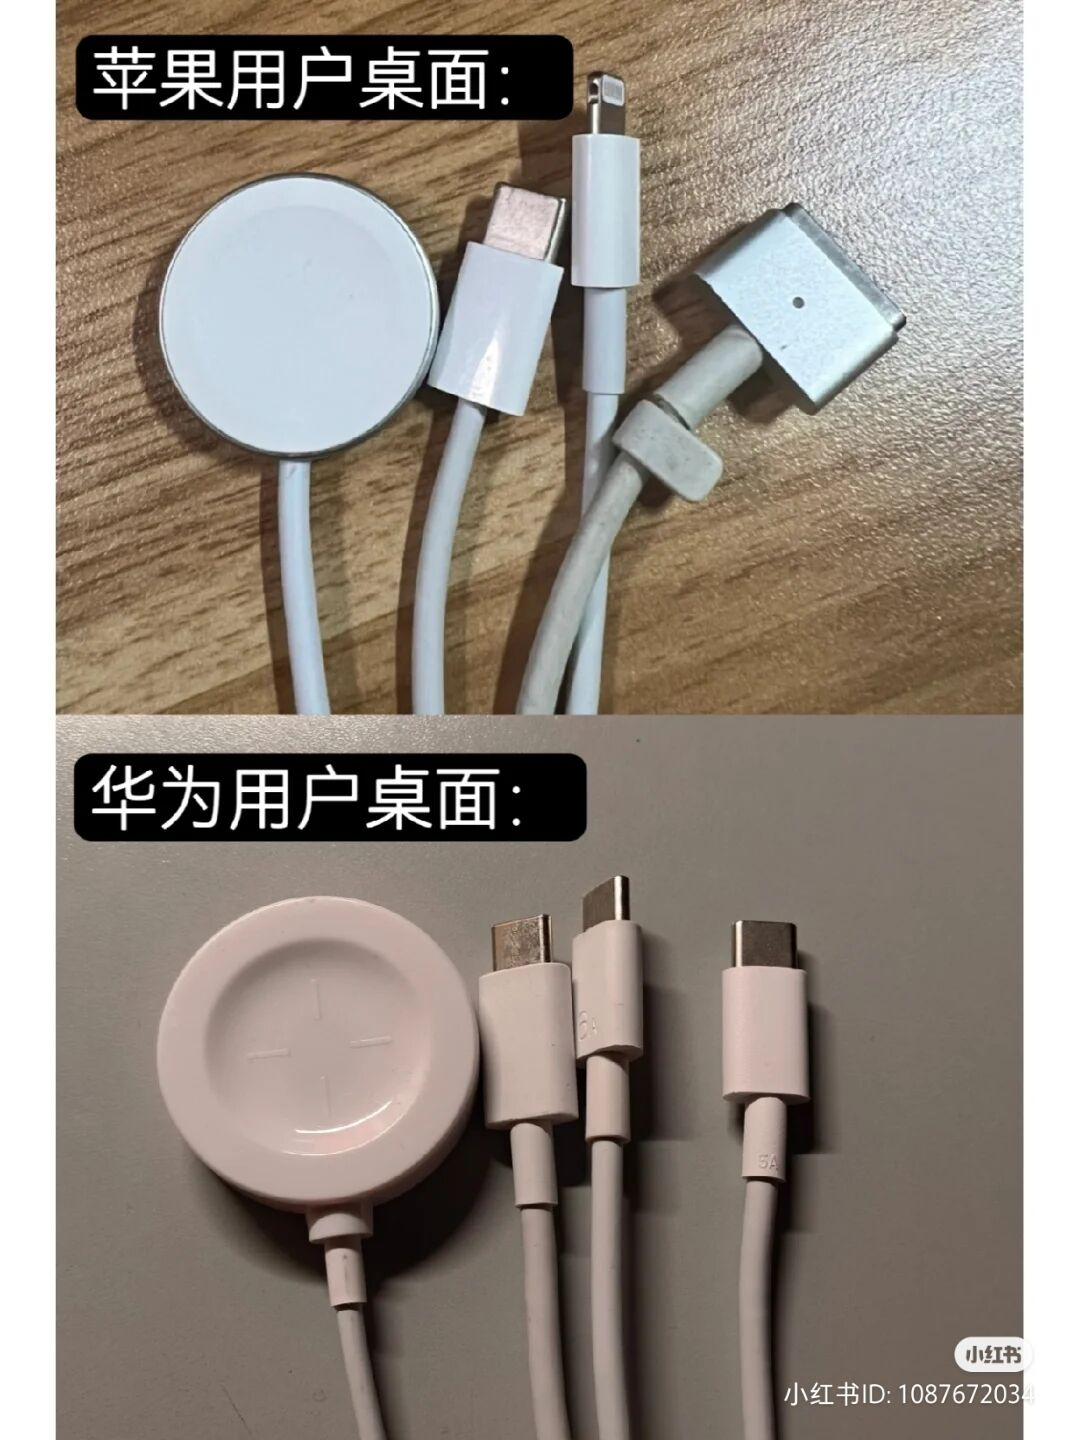
\includegraphics[scale=0.135]{figures/interface1.jpg}
        \end{minipage}
        \begin{minipage}{0.48\textwidth}
            \centering
            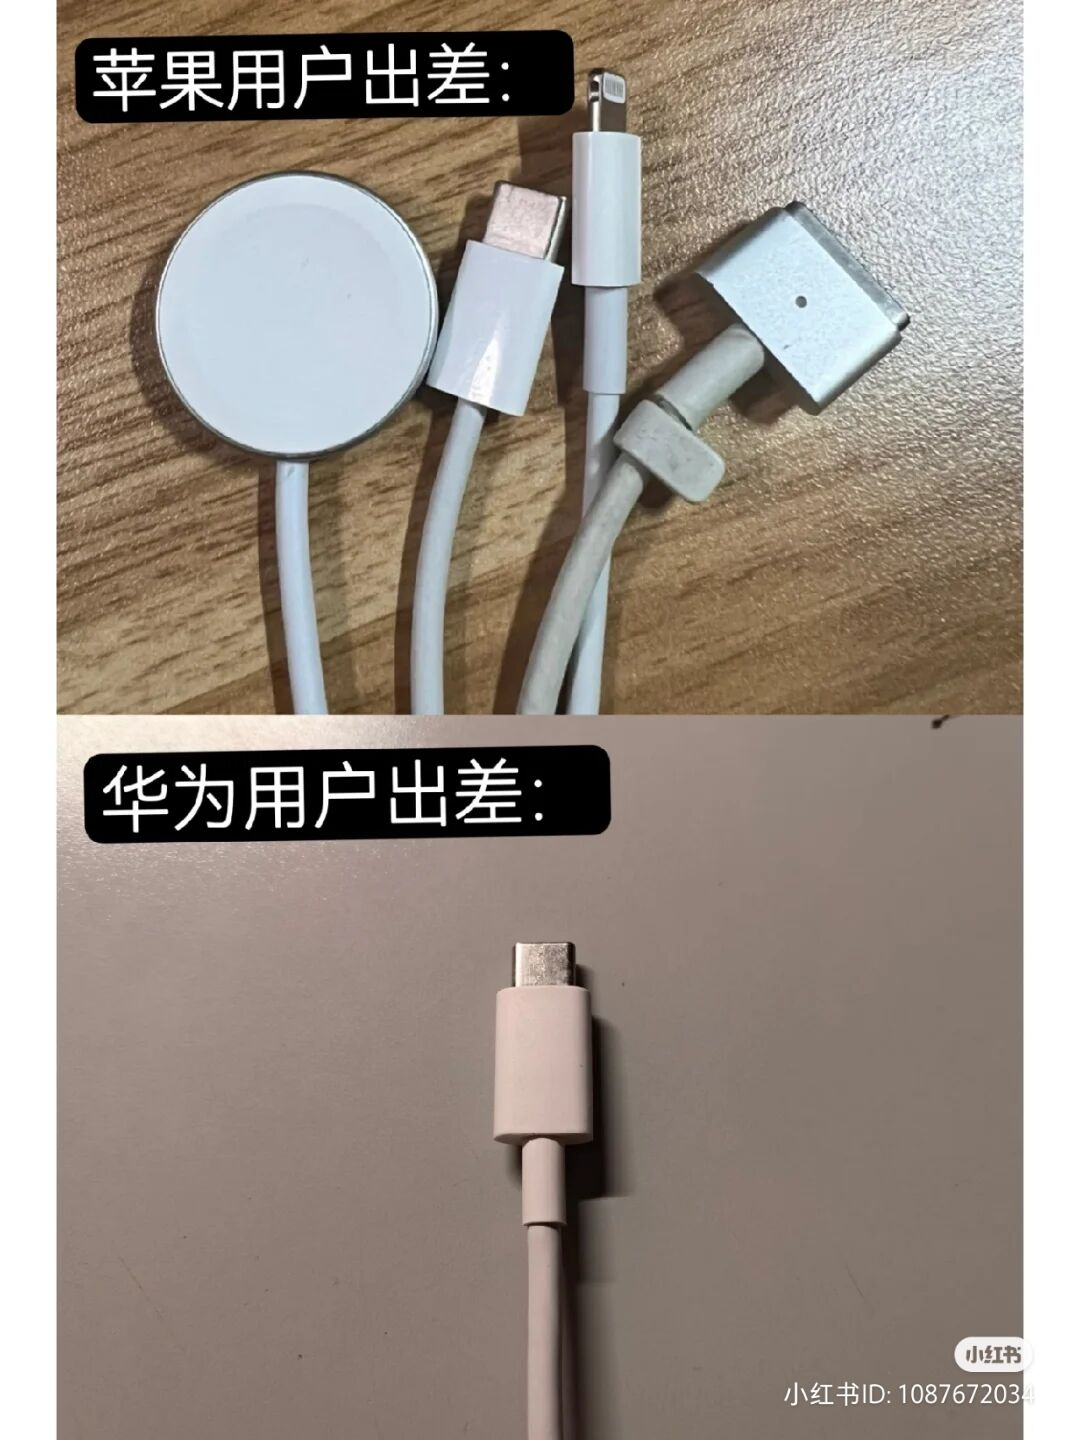
\includegraphics[scale=0.135]{figures/interface2.jpg}
        \end{minipage}
    \end{figure}
\end{frame}

\begin{frame}{Data }
\end{frame}